\section{Цель работы}

\begin{enumerate}
	\item Установить и настроить пакет GPG 2
	\item Создать набор ключей в Kleopatra
	\item Экспортировать свой ключ, импортировать ключ другого участника эксперимента
	\item Зашифровать файл и отправить другому человеку, расшифровать чужой файл
	\item Выполнить те же пункты, используя консольный интерфейс
\end{enumerate}

\section{Ход работы}

\subsection{Использование GPG с помощью интерфейса Kleopatra}

Установим необходимые инструменты:

\begin{verbatim}
bodrik@Bodrik-N53SV:~$ sudo apt-get install kleopatra gnupg2
\end{verbatim}

Запустим Kleopatra. Перед нами появится главное окно:

\begin{figure}[H]
	\centering
	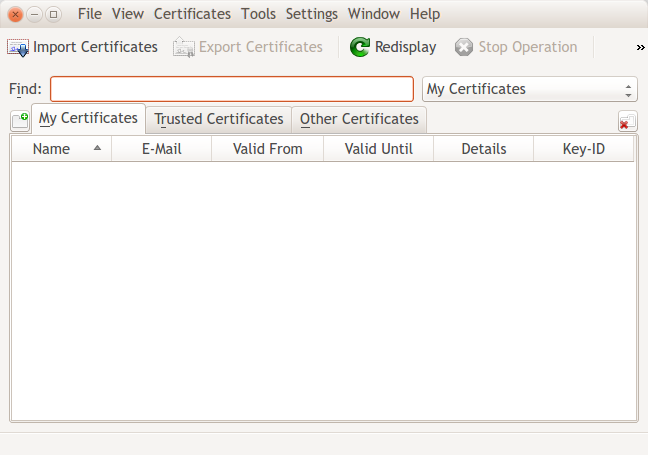
\includegraphics[width=0.8\textwidth]{images/1.png}
	\caption{Главное окно программы Kleopatra}
\end{figure}

Через меню <<Файл>> запустим мастер создания ключа

\begin{figure}[H]
	\centering
	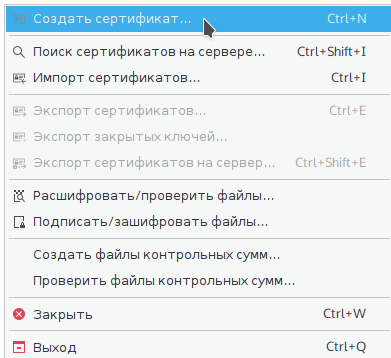
\includegraphics[width=0.7\textwidth]{images/0.png}
	\caption{Меню <<Файл>>}
\end{figure}

В данной работе нас интересуют ключи PGP, поэтому выберем первый пункт.

\begin{figure}[H]
	\centering
	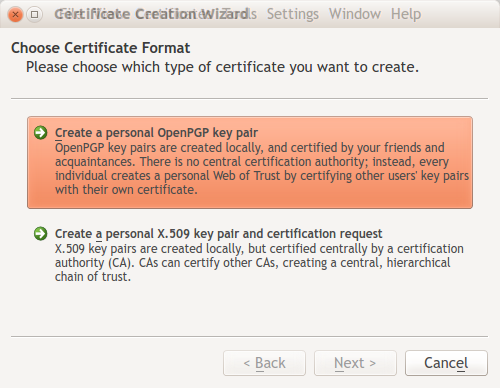
\includegraphics[width=0.8\textwidth]{images/2.png}
	\caption{Создание ключа}
\end{figure}

Укажем свои реквизиты

\begin{figure}[H]
	\centering
	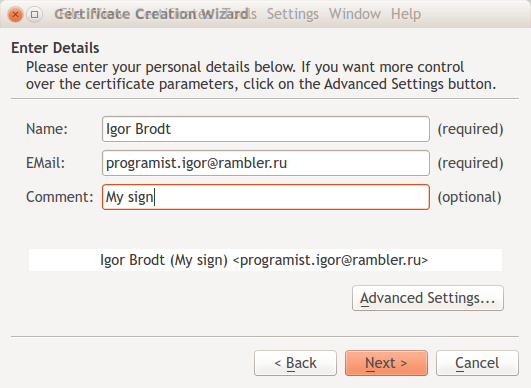
\includegraphics[width=0.8\textwidth]{images/3.png}
	\caption{Создание ключа}
\end{figure}

В дополнительных параметрах проверим, что используются достаточная длина ключа, а также ограничим срок годности ключа.

\begin{figure}[H]
	\centering
	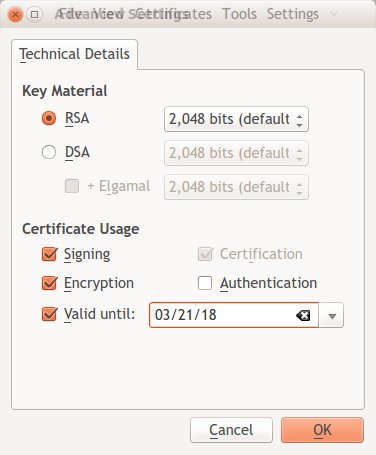
\includegraphics[width=0.6\textwidth]{images/4.png}
	\caption{Создание ключа}
\end{figure}

\begin{figure}[H]
	\centering
	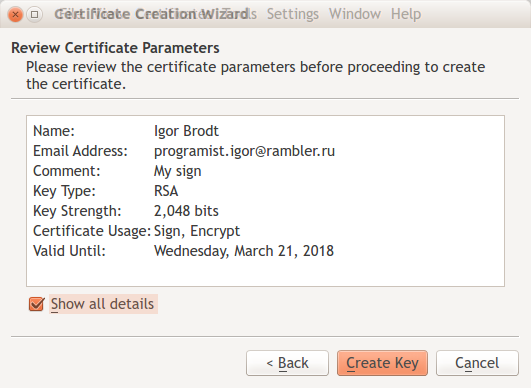
\includegraphics[width=0.6\textwidth]{images/5.png}
	\caption{Сводные параметры создания ключа}
\end{figure}

Введем пароль

\begin{figure}[H]
	\centering
	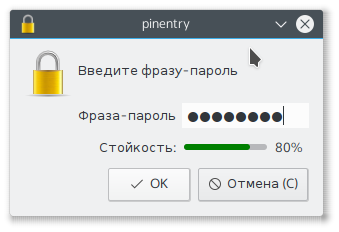
\includegraphics[width=0.5\textwidth]{images/6.png}
	\caption{Создание ключа}
\end{figure}

\begin{figure}[H]
	\centering
	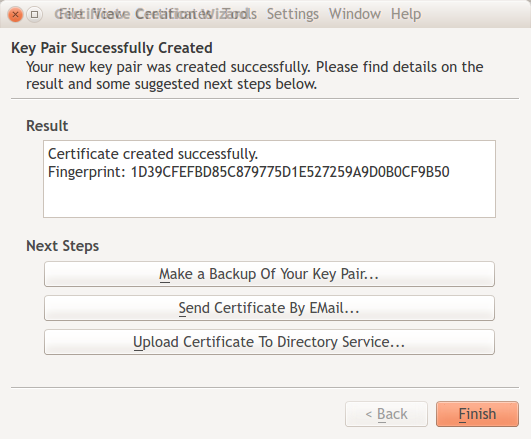
\includegraphics[width=0.8\textwidth]{images/7.png}
	\caption{Создание ключа}
\end{figure}

Наш ключ появился в списке

\begin{figure}[H]
	\centering
	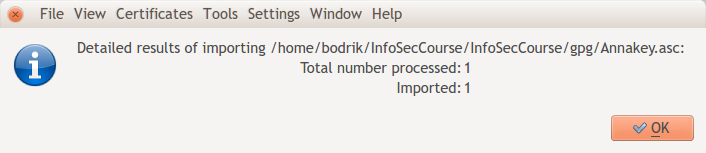
\includegraphics[width=0.8\textwidth]{images/8.png}
	\caption{Ключи}
\end{figure}

Получим сертификат от другого участника эксперимента, импортируем его.

\begin{figure}[H]
	\centering
	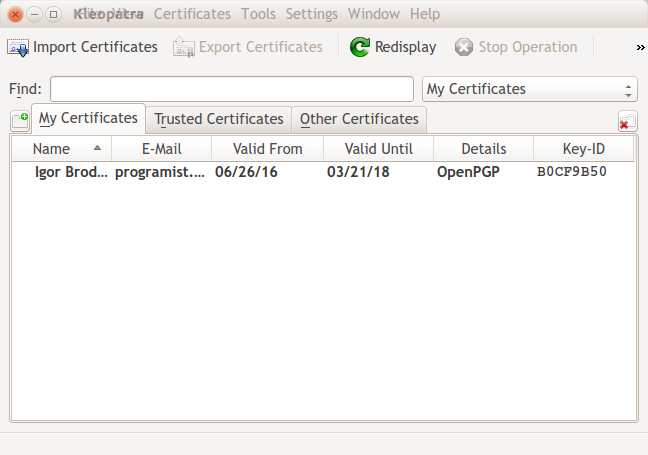
\includegraphics[width=0.8\textwidth]{images/9.png}
	\caption{Импорт сертификата}
\end{figure}

Видим его в списке

\begin{figure}[H]
	\centering
	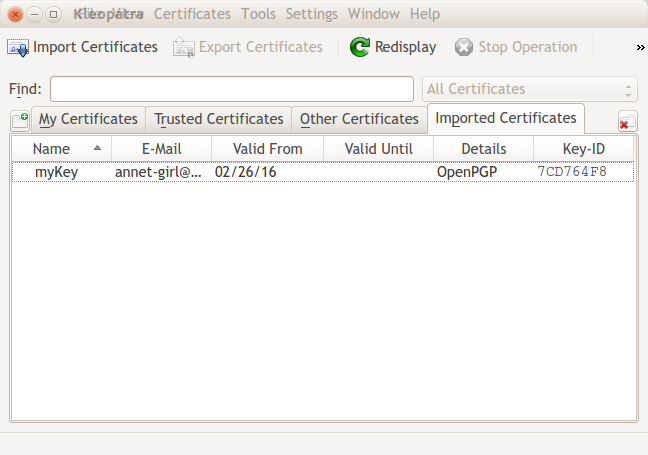
\includegraphics[width=0.8\textwidth]{images/10.png}
	\caption{Сертификаты}
\end{figure}

Зашифруем файл. Для удобства обмена включим использование текстового представления зашифрованных данных.

\begin{figure}[H]
	\centering
	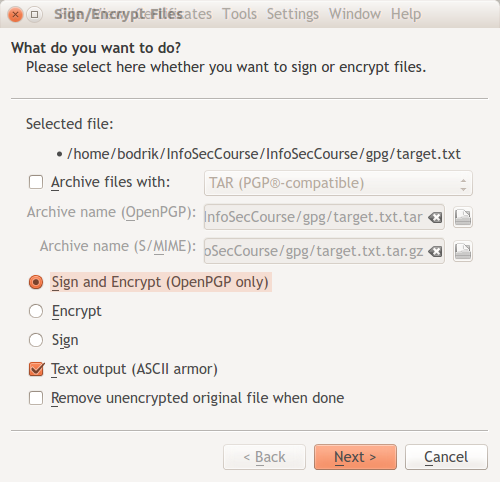
\includegraphics[width=0.8\textwidth]{images/11.png}
	\caption{Шифрование}
\end{figure}

Выберем свой и чужой ключ

\begin{figure}[H]
	\centering
	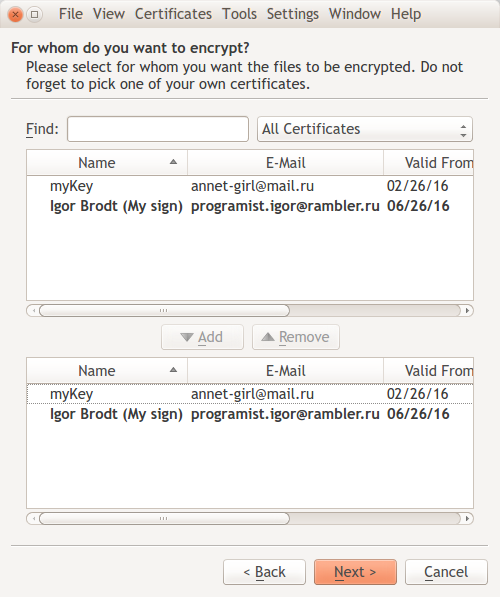
\includegraphics[width=0.8\textwidth]{images/12.png}
	\caption{Шифрование}
\end{figure}

Выберем открытый ключ, с помощью которого будем шифровать

\begin{figure}[H]
	\centering
	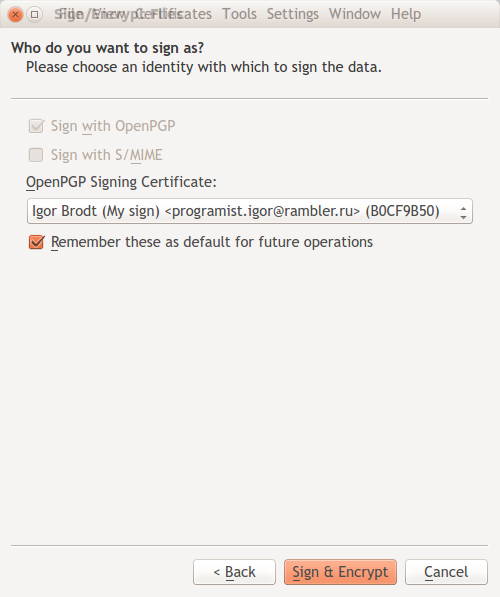
\includegraphics[width=0.8\textwidth]{images/13.png}
	\caption{Шифрование}
\end{figure}

Сообщение об успехе

\begin{figure}[H]
	\centering
	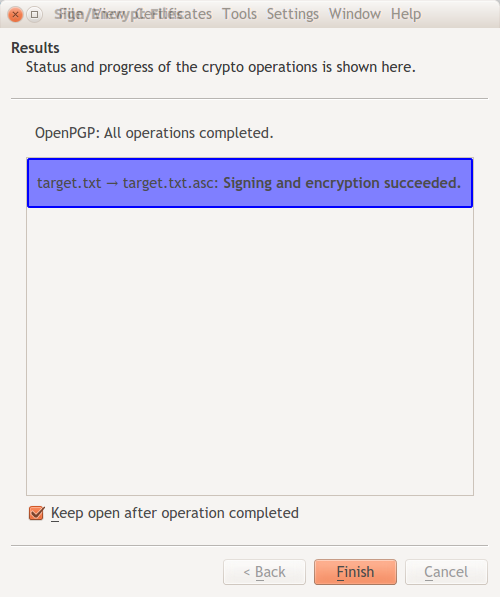
\includegraphics[width=0.8\textwidth]{images/14.png}
	\caption{Шифрование}
\end{figure}

Так выглядит зашифрованный файл

\begin{figure}[H]
	\centering
	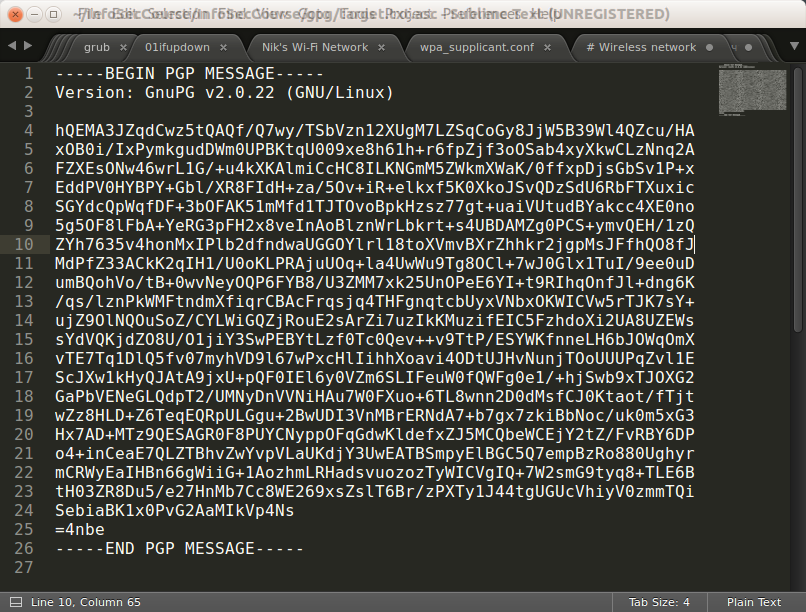
\includegraphics[width=0.8\textwidth]{images/15.png}
	\caption{Зашифрованный файл}
\end{figure}

Теперь попробуем расшифровать файл, для этого запустим мастер из меню <<Файл>>.

\begin{figure}[H]
	\centering
	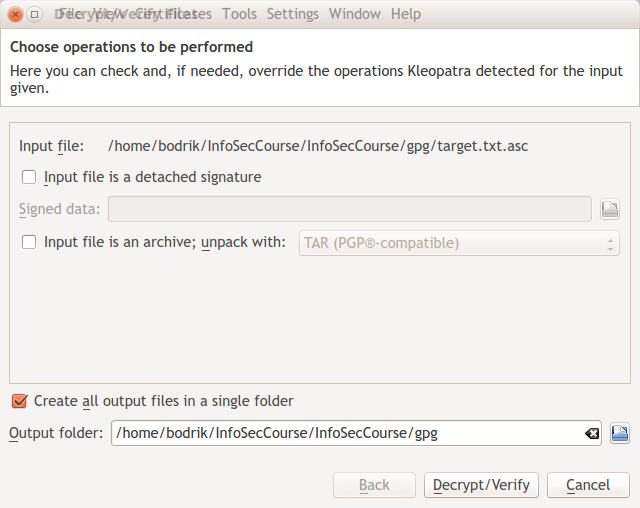
\includegraphics[width=0.8\textwidth]{images/16.png}
	\caption{Расшифровка}
\end{figure}

\begin{figure}[H]
	\centering
	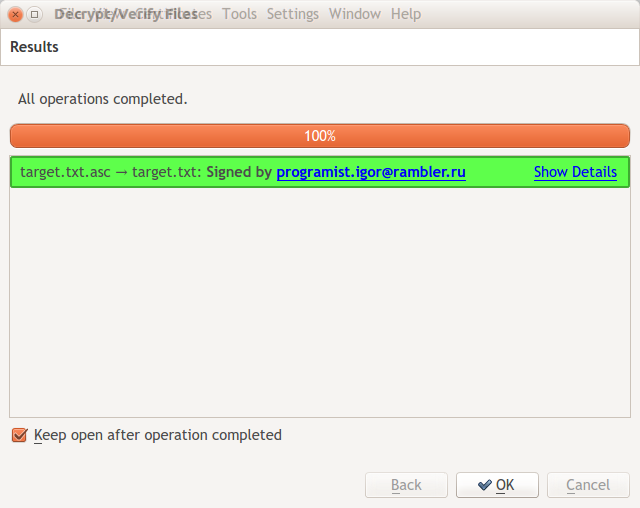
\includegraphics[width=0.8\textwidth]{images/17.png}
	\caption{Расшифровка}
\end{figure}

Ниже представлено расшифрованное изображение

\begin{figure}[H]
	\centering
	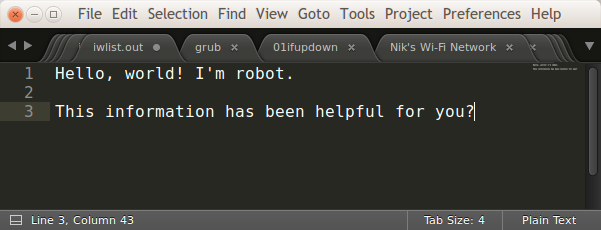
\includegraphics[width=0.8\textwidth]{images/18.png}
	\caption{Расшифрованное изображение}
\end{figure}

\subsection{Использование GPG с помощью консольного интерфейса}

Эксперименты будут проводиться на другой машине. Попробуем вывести список ключей.

\begin{verbatim}  
bodrik@Bodrik-N53SV:~$ gpg2 --list-keys
/home/bodrik/.gnupg/pubring.gpg
-------------------------------
pub   4096R/1636CC92 2011-09-02
uid                  Double GIS (Repository 2GIS) <tech@2gis.ru>

pub   2048R/B0CF9B50 2016-06-26 [expires: 2018-03-21]
uid                  Igor Brodt (My sign) <programist.igor@rambler.ru>

pub   2048R/7CD764F8 2016-02-25
uid                  myKey <annet-girl@mail.ru>
sub   2048R/4BECA6BD 2016-02-25
\end{verbatim}

Cоздадим новый ключ.

\begin{verbatim}
bodrik@Bodrik-N53SV:~$ gpg2 --gen-key
gpg (GnuPG) 2.0.22; Copyright (C) 2013 Free Software Foundation, Inc.
This is free software: you are free to change and redistribute it.
There is NO WARRANTY, to the extent permitted by law.

Please select what kind of key you want:
   (1) RSA and RSA (default)
   (2) DSA and Elgamal
   (3) DSA (sign only)
   (4) RSA (sign only)
Your selection? 1
RSA keys may be between 1024 and 4096 bits long.
What keysize do you want? (2048) 
Requested keysize is 2048 bits
Please specify how long the key should be valid.
         0 = key does not expire
      <n>  = key expires in n days
      <n>w = key expires in n weeks
      <n>m = key expires in n months
      <n>y = key expires in n years
Key is valid for? (0) 3m
Key expires at Сб. 24 сент. 2016 19:11:08 MSK
Is this correct? (y/N) y

GnuPG needs to construct a user ID to identify your key.

Real name: Igor Brodt
Email address: programist.igor@rambler.ru
Comment: Key2
You selected this USER-ID:
    "Igor Brodt (Key2) <programist.igor@rambler.ru>"

Change (N)ame, (C)omment, (E)mail or (O)kay/(Q)uit? O
You need a Passphrase to protect your secret key.

We need to generate a lot of random bytes. It is a good idea to perform
some other action (type on the keyboard, move the mouse, utilize the
disks) during the prime generation; this gives the random number
generator a better chance to gain enough entropy.
We need to generate a lot of random bytes. It is a good idea to perform
some other action (type on the keyboard, move the mouse, utilize the
disks) during the prime generation; this gives the random number
generator a better chance to gain enough entropy.
gpg: key 1C0637E6 marked as ultimately trusted
public and secret key created and signed.

gpg: checking the trustdb
gpg: 3 marginal(s) needed, 1 complete(s) needed, PGP trust model
gpg: depth: 0  valid:   2  signed:   0  trust: 0-, 0q, 0n, 0m, 0f, 2u
gpg: next trustdb check due at 2016-09-24
pub   2048R/1C0637E6 2016-06-26 [expires: 2016-09-24]
      Key fingerprint = 3832 6829 0846 9C94 47A0  F80F 53EE FFF9 1C06 37E6
uid                  Igor Brodt (Key2) <programist.igor@rambler.ru>
sub   2048R/037DAF12 2016-06-26 [expires: 2016-09-24]

\end{verbatim}

В списке появился новый ключ:

\begin{verbatim}
bodrik@Bodrik-N53SV:~$ gpg2 --list-keys
/home/bodrik/.gnupg/pubring.gpg
-------------------------------
pub   4096R/1636CC92 2011-09-02
uid                  Double GIS (Repository 2GIS) <tech@2gis.ru>

pub   2048R/B0CF9B50 2016-06-26 [expires: 2018-03-21]
uid                  Igor Brodt (My sign) <programist.igor@rambler.ru>

pub   2048R/7CD764F8 2016-02-25
uid                  myKey <annet-girl@mail.ru>
sub   2048R/4BECA6BD 2016-02-25

pub   2048R/1C0637E6 2016-06-26 [expires: 2016-09-24]
uid                  Igor Brodt (Key2) <programist.igor@rambler.ru>
sub   2048R/037DAF12 2016-06-26 [expires: 2016-09-24]

\end{verbatim}

Экспортируем его.

\begin{verbatim}
bodrik@Bodrik-N53SV:~$ gpg2 --export --armor 1C0637E6
-----BEGIN PGP PUBLIC KEY BLOCK-----
Version: GnuPG v2.0.22 (GNU/Linux)

mQENBFdv/vwBCADDczUydkKnzUoYJttIE+Qd/QMlXIF6urNQrxYDvSiwGwUi36uU
UNWKJCrgw2H/U9jTYMGxi58jgMPEv0S5K4+BNB0AXOfAltInXGDXCMC+UNUwyhY3
GSHu1Q5Z4Qyrf3ctPq/VTXU2xqSIIgUhG0RqzlIBDpdvYYglo6pExlwHnrU4KfT+
JC5M0Yt8HM05NWqmLWr8b4y8WMqd5jXJd6cz2euNEhyCnD3IJCi5tDVREMfFYpKP
SYq57pwuDUP4bP+5K8kuzQeCsONDnVtousvoqQEmDtsIta2qXl5mmqb7hdbjgQz1
dLSHST9P+dPl4vXiBpMy4VyLOZ455Lddun2NABEBAAG0Lklnb3IgQnJvZHQgKEtl
eTIpIDxwcm9ncmFtaXN0Lmlnb3JAcmFtYmxlci5ydT6JAT8EEwECACkFAldv/vwC
GwMFCQB2pwAHCwkIBwMCAQYVCAIJCgsEFgIDAQIeAQIXgAAKCRBT7v/5HAY35t3r
CACNOf8bvnZfGBuOd5M53X2FVvSDoEdd0XfZ777ofs/Rf1UU3r6jChjpHF5c3Gh8
u7LyBj3NcUZkyag+MB/KeHkT2FA/qbz/W0KD5Pm/q+uoEJJnbMM6e4bIg+k6+N/R
VtAHEoBC1qC+gtVw+4UbJ2qPucKXDvHttZn6YBTU7PnnbOYuIKDE7ZlfcRYwBbAG
aKq3uhZx3+oPSBiyP9dVXb08zktzIvgW4PMXpCxCEnr0clFOEM+uSK7lflJrCjUa
yJNEE/9KHuGQCkBiu4N/+CAW5ar31Bi5LDQRuQg4BFIUV+fZhzfx12pTF6aotMQZ
lGBBzve1kQieh+C8dJc5C6dguQENBFdv/vwBCAC1tYCfH7Rim3kTAKeBICKNYtd5
sFTf8wus0U/g6AnLr9SOLNDevpge0zXm0NkMo6ySFSc5EIix2IeZINKWCf8Mv7uR
G77p5lqqJyV1dZXlH8FiJ5XYZd98YcLvVv09p+35luOpWfQ9zH5zJBp44Ry777Yb
yQ3FqAobD/D0cpaJM68Mu4dkxPOKAEDRMgs3MbRStsPN1we/gAPewQHCb2EZNGaO
638OvOP5q1Z41pCUQvnDqb5pMe+ihShwREGGVmPI9rpmCdsaL3J2YH77gDbwxESj
SW0X2y59Xk38A5VqLr/4v3/Tl0opPk5ljoH4Uss5G5dMhy6fczapXK4CAa8PABEB
AAGJASUEGAECAA8FAldv/vwCGwwFCQB2pwAACgkQU+7/+RwGN+YM7Qf/QeL9RE2J
3Vg2tQo6FgjRJ16EL+T/6TcA8nAluvR5iAdD3Qvmyow/FF75zNFMtY0VIhbpj9hI
bpoImoXaH7TjBxU4hdWeemRnyC94UdRsxv3Vsg7I5m8II2xpRVlkpHQOh0SKdKTA
tve5AhpQV4mVpdRy6+ypjTdON03zsCB1hNGdQ1A4D3V7BW5TlIsL0h8kPQdXjKg6
BRDqaG0+VA2w6//Ugblk9NY6h31XYjq55YgJNHFV99/Sr5xiAEpnpDDGfDvDUEb2
juQC81bGKBQbb3M1p8n73Yy/uG8iJCspRTj8hw23h9VR5Kd2ZagejT4ddOpAsEfi
0S5+XhoYjjszQg==
=bgTR
-----END PGP PUBLIC KEY BLOCK-----

\end{verbatim}

Попробуем зашифровать файл.

Импортируем ключ:

\begin{verbatim}  
bodrik@Bodrik-N53SV:~$ gpg2 --import /home/bodrik/InfoSecCourse/InfoSecCourse/gpg/Annakey.asc
gpg: key 7CD764F8: "myKey <annet-girl@mail.ru>" not changed
gpg: Total number processed: 1
gpg:              unchanged: 1
\end{verbatim}

Запустим шифрование:

\begin{verbatim}
bodrik@Bodrik-N53SV:~$ gpg2 --armor --encrypt /home/bodrik/InfoSecCourse/InfoSecCourse/gpg/target2.txt
You did not specify a user ID. (you may use "-r")

Current recipients:

Enter the user ID.  End with an empty line: 1C0637E6

Current recipients:
2048R/037DAF12 2016-06-26 "Igor Brodt (Key2) <programist.igor@rambler.ru>"

Enter the user ID.  End with an empty line: 7CD764F8
gpg: 4BECA6BD: There is no assurance this key belongs to the named user

pub  2048R/4BECA6BD 2016-02-25 myKey <annet-girl@mail.ru>
 Primary key fingerprint: 20D1 A3C8 58A9 CA18 7BD0  CBBE 44D1 1089 7CD7 64F8
      Subkey fingerprint: D8A9 6850 A1F3 2986 EBCD  351F 1983 43C2 4BEC A6BD

It is NOT certain that the key belongs to the person named
in the user ID.  If you *really* know what you are doing,
you may answer the next question with yes.

Use this key anyway? (y/N) y

Current recipients:
2048R/4BECA6BD 2016-02-25 "myKey <annet-girl@mail.ru>"
2048R/037DAF12 2016-06-26 "Igor Brodt (Key2) <programist.igor@rambler.ru>"

Enter the user ID.  End with an empty line: 

\end{verbatim}

В директории появился новый файл

\begin{verbatim}
target2.txt.asc
\end{verbatim}